% Main document of the project, this will include all the other parts involving the documentation...

\documentclass[a4paper]{article}
\usepackage[utf8]{inputenc}
\usepackage[T1]{fontenc}

%% Sets page size and margins
\usepackage[a4paper,top=3cm,bottom=2cm,left=3cm,right=3cm,marginparwidth=1.75cm]{geometry}

%% Useful packages
\usepackage{amsmath}
\usepackage{floatrow}
\usepackage{graphicx}
\graphicspath{ {./images/} }
\usepackage[colorinlistoftodos]{todonotes}
\usepackage[colorlinks=true, allcolors=blue]{hyperref}
\usepackage{amsmath}
\usepackage{chngcntr}
\usepackage{wrapfig}
\usepackage{caption}
\usepackage{subcaption}
\usepackage{listings}
\usepackage{placeins}
\usepackage{multicol}
\usepackage{verbatim}
\usepackage[sorting=none]{biblatex}
\usepackage{csvsimple}
\usepackage{xcolor}
\usepackage{listings}
\usepackage[spanish]{babel}
\renewcommand\spanishtablename{Tabla}
\selectlanguage{spanish}

\captionsetup[table]{position=bottom}
\usepackage[table]{xcolor}

\renewcommand{\lstlistingname}{Código}% 
\renewcommand{\lstlistlistingname}{Lista de código}% List of Listings -> List of Algorithms

% extracted from internet: https://timmurphy.org/2014/01/27/displaying-code-in-latex-documents/
\definecolor{lbcolor}{rgb}{0.93,0.93,0.93}
\lstset{  
    frame=tb, % draw a frame at the top and bottom of the code block
    tabsize=4, % tab space width
    showstringspaces=false, % don't mark spaces in strings
    numbers=left, % display line numbers on the left
    commentstyle=\color{green}, % comment color
    keywordstyle=\color{blue}, % keyword color
    stringstyle=\color{red},
    backgroundcolor=\color{lbcolor}
}

\definecolor{main-color}{rgb}{0.6627, 0.7176, 0.7764}
\definecolor{back-color}{rgb}{0.1686, 0.1686, 0.1686}
\definecolor{string-color}{rgb}{0.3333, 0.5254, 0.345}
\definecolor{key-color}{rgb}{0.8, 0.47, 0.196}
\lstdefinestyle{idlstyle}
{
    language = C++,
    keywordstyle = {\color{key-color}},
    keywordstyle = [3]{\color{blue}},
    otherkeywords = {in, int ,interface, out, inout},
    morekeywords = [3]{in, out, inout}
}

\setcounter{secnumdepth}{3}
\setcounter{tocdepth}{3}

% \title{Integrating COMPSs and OmpSs Programming Models to support distributed heterogeneous computing environments}
\title{Integrating COMPSs and OmpSs Programming Models to support distributed heterogeneous computing environments}
\author
{
Marc Domínguez de la Rocha
\and
Rosa M. Badia
\and
Jorge Ejarque
}
\date{Febrero 2019}

\bibliography{bibliography} 
\begin{document}

\maketitle

\newpage
\renewcommand{\contentsname}{Índice}
\tableofcontents
\newpage

%% La siguiente seccion enmarca el contexto
% que envuelve al proyecto y de alguna
% manera el por qué
\section{Contexto}

Hoy en día se tiende a tener distintos recursos de cómputo en un solo dispositivo, por ejemplo, en un teléfono móvil ya tenemos al menos un procesador y una tarjeta gráfica, pero no tan sólo en el ámbito más cotidiano (aunque no nos demos cuenta), sino que en los más profesionales y especializados está siendo también cada vez más común la heterogeneidad de los recursos de computación. 
\par\bigskip

El proyecto pretende facilitar la gestión de estos recursos de computación en entornos distribuidos, brindando un método robusto y eficiente para programar aplicaciones en estos entornos.
%Quienes son los actores? Quien se beneficia?


\subsection{Introducción}

Este proyecto es un Trabajo de Fin de Grado del Grado en Ingeniería Informática, especializado en el área de Ingeniería de Computadores. El grado es impartido por la \textit{Facultat d'Informàtica de Barcelona (FIB)} centro perteneciente a la \textit{Universitat Politècnica de Catalunya (UPC)}. 
\par\bigskip

El proyecto se desarrollará conjuntamente con el \textit{Barcelona Supercomputing Center (BSC)}, estudiaremos como podemos integrar los modelos de programación \textit{COMPSs} y \textit{OmpSs} para alcanzar este objetivo, implementaremos un prototipo y evaluaremos su rendimiento y características deseadas. 
%Indagar en cuales son estas caracteristicas? 

\subsection{Actores}

Los actores en este proyecto serán las personas que tomen parte en él, ya sea de manera directa o indirecta. Con esto quiero decir, que tanto las personas que tomen parte en el desarrollo \textit{per se} como las personas que se nutran de este, serán los actores.

\begin{itemize}
 \item \textbf{Desarrollador:} La figura del desarrollador \textbf{debe} ser la persona que trabaje de manera más directa en el proyecto. En este proyecto únicamente habrá un desarrollador que ha elaborado la documentación que leerás a continuación y dará forma a los objetivos tangibles del proyecto.  
 \item \textbf{Director y codirector:} Pese a que el desarrollador tendrá el papel principal en el proyecto, el director y el codirector le guiarán en el camino abierto que es el desarrollo del proyecto. Se establecerán reuniones de seguimiento donde serán capaces de hacer un correcto supervisamiento de las actividades propuestas para el proyecto.
 \item \textbf{Barcelona Supercomputing Center:} De manera directa el centro otorga al desarrollador un lugar de trabajo y un equipo informático. Por otra parte, cuenta con el soporte por parte de los equipos de desarrollo de \textit{COMPSs} (del cual forma parte el desarrollador) y de \textit{OmpSs} para cualquier incidencia relacionada con su \textit{software} y derivados.
 \item \textbf{Beneficiarios:} \textit{COMPSs} es utilizado para proyectos europeos en los cuales el \textit{BSC} toma parte, el proyecto podrá ser útil para algunos de ellos, además todo departamento del \textit{BSC} que utilice \textit{COMPSs} para el desarrollo de aplicaciones podrá utilizarlo.
\end{itemize}

\section{Estado del arte}

%check si te estas patillando lo de ``centenares''
Existen centenares de modelos de programación, véanse \textit{OpenMP}, \textit{OmpSs}, \textit{MPI}, \textit{COMPSs} y un largo etcétera. De alguna manera el objetivo en común fue y es aprovechar los cada vez más abundantes recursos en las máquinas, que finalmente no sólo han crecido en abundancia si no en diversidad. La filosofía sigue siendo la misma, sacar el mayor rendimiento posible a nuestras máquinas. 
\par\bigskip

Para esto son necesarios modelos de programación que nos den la posibilidad de utilizar los recursos y nos ayuden a explotar la posible sinergia entre estos en ciertas aplicaciones. 
\par\bigskip

La diferencia más elemental entre los modelos, es en como se gestiona la memoria, o bien como la memoria está dispuesta en el modelo. Con \textit{shared memory} (\textit{OpenMP}, \textit{OmpSs}...), se aprovecha que el conjunto de hilos de ejecución (\textit{threads}) comparten la memoria, con \textit{distributed memory} (\textit{MPI}...) que se utilizan diferentes procesos con la posibilidad de que estos estén distribuidos entre distintos nodos, existen también modelos como \textit{CUDA} y \textit{OpenCL} que transfieren memoria de la \textit{CPU} a la memoria del acelerador en cuestión.
\par\bigskip

La integración de los modelos propuestos \textit{COMPSs} y \textit{OmpSs} nos otorgará la posibilidad de utilizar todos los recursos de la máquina, a continuación se ahonda en las características de ambos.

\subsection{COMPSs}

\textit{COMPSs} es desarrollado por el grupo \textit{Workflows and Distributed Computing} que pertenece al departamento de \textit{CS - Computer Science}.
\par\bigskip

\textit{COMPSs} es un modelo de programación para entornos distribuidos basado en la generación de tareas, el objetivo es hacer más sencilla la programación de aplicaciones y su ejecución en entornos distribuidos (clústers y \textit{clouds}, por ejemplo)\cite{badia2015comp}.La generación de tareas la efectua un programa principal ejecutado en secuencial, las tareas se especifican mediante la anotación de las funciones que se deseen, en tiempo de ejecución se genera un grafo de tareas y se detectan las dependencias entre estas para ejecutarlas en el orden correcto. Dado que está preparado para ejecutarse en entornos distribuidos también se detecta cuando son necesarias transferencias entre nodos.   \par\bigskip

Para facilitar más aún el uso del modelo, está dotado de un sistema de \textit{runtime} compuesto por un \textit{master} y un conjunto de \textit{workers}, el \textit{runtime} coexiste con la aplicación. Se encarga de detectar las dependencias que puedan surgir entre las tareas que genera el programa principal y las ejecuta a medida que las dependencias se resuelven. 
%\par\bigskip

\subsubsection{Modelo de programación} 
\label{compss_pm}

El \textit{runtime} de \textit{COMPSs} está implementado en \textit{Java} por lo cuál se soporta dicho lenguaje, además se desarrollaron los \textit{bindings} de \textit{Python}\cite{tejedor2017pycompss} y \textit{C/C++} para facilitar el portaje de aplicaciones en estos lenguajes a \textit{COMPSs}. 
\par\bigskip

Dicho esto, centraremos nuestros esfuerzos en \textit{C} y \textit{C++}. Para desarrollar una aplicación de \textit{COMPSs} en \textit{C/C++} necesitamos el programa principal (ejecutado en secuencial), una interfaz que especificará las funciones que \textit{a posteriori} serán tareas, y el código que realmente implementan estas tareas. 
\par\bigskip

Veamos en orden de enumeración ejemplos de los componentes de una aplicación.

%EJEMPLO INTERFACE
\begin{lstlisting}[caption={Interfaz de la aplicación 'ejemplo'.},captionpos=b, label={lst:ejemplo.idl}, style=idlstyle]
interface ejemplo {
    void funcionEjemplo(in int a, out int[a] array_a);
};
\end{lstlisting}

La interfaz de la imagen superior define una función llamada funcionEjemplo con un parámetro de entrada y uno de salida, las palabras clave \textit{in} y \textit{out} respectivamente otorgan estas propiedades a los parámetros, también se puede combinar con \textit{inout}. Cualquier llamada a la función será ejecutada como tarea.\smallskip

%EJEMPLO MASTER CODE
\begin{lstlisting}[caption={Fracción del código del programa principal}, captionpos=b, label={lst:ejemplo.cc}, language=C++]
    compss_on();

    int a = 10;
    int* array_a;

    funcionEjemplo(a, array_a);

    compss_wait_on(array_a);

    compss_off();
\end{lstlisting}

Esta imagen muestra el código del programa principal de manera reducida. Es tan sencillo como prometía, encendemos el \textit{runtime} de \textit{COMPSs}, preparamos los parámetros de la función, ejecutamos y finalmente esperamos a los parámetros de salida y apagamos el \textit{runtime}. \smallskip

\begin{lstlisting}[caption={Implementación de la función 'funcionEjemplo'}, captionpos=b, label={lst:ejemplo-functions.cc}, language=C++]
void funcionEjemplo(int a, int array_a[]) {
    for (int i = 0; i < a; ++i) {
        array_a[i] = a;
    }
}
\end{lstlisting}

Las tareas se implementan como funciones que serán ejecutadas por los workers. Salvo convenciones en los nombres de los ficheros para hacer la compilación de la aplicación esto es todo lo necesario para desarrollar una aplicación en \textit{COMPSs} de \textit{C/C++}.

\begin{comment}
\subsubsection{Compilación}

Para compilar la aplicacion en \textit{COMPSs} de \textit{C/C++}, 

\begin{figure}[H]
    \centering
    \caption{Proceso de compilado de una aplicación COMPSs C/C++}
%    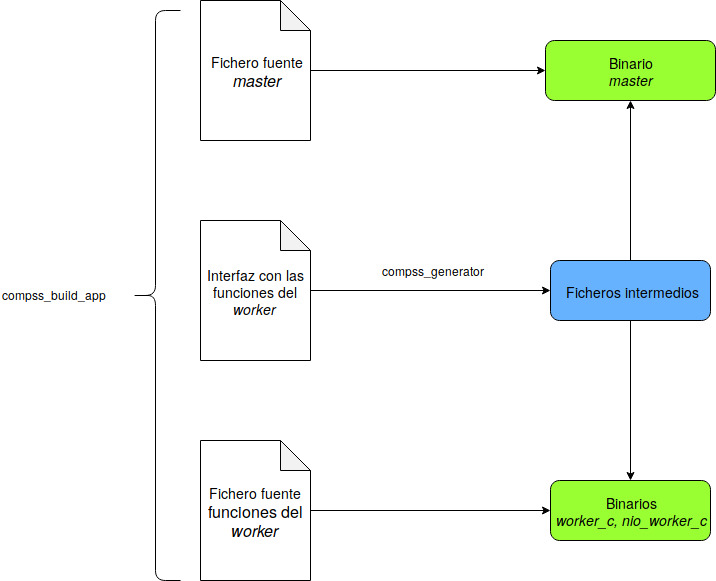
\includegraphics[width=\textwidth]{proceso_compilado.jpg}
    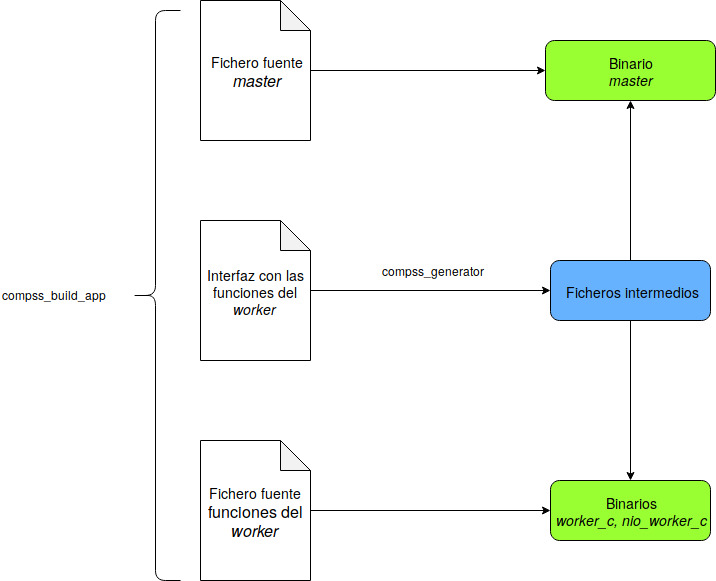
\includegraphics[scale=0.5]{proceso_compilado.jpg}
    \label{fig:proceso_compilado}
\end{figure}
\end{comment}

\subsubsection{Modelo de ejecución\label{modeloejecucion}}

El modelo de ejecución es sencillo, muy similar al modelo \textit{thread-pool}, al iniciar el \textit{runtime} se levanta el \textit{master} y un conjunto de \textit{workers}, a medida que se vayan generando tareas se estudiará qué \textit{workers} están libres y si cumplen los requisitos para ejecutar dicha tarea, y en ese caso la ejecutarán. 

\begin{figure}[H]
    \centering 
    \caption{Modelo de ejecución, basado en la aplicación 'ejemplo'.}
    %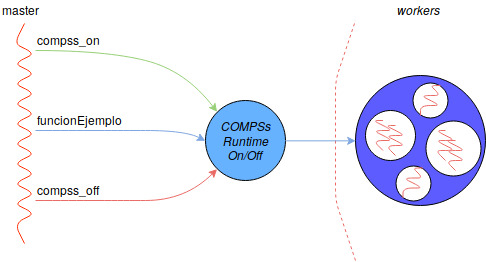
\includegraphics[width=\textwidth]{sta-masterworker.jpg}
    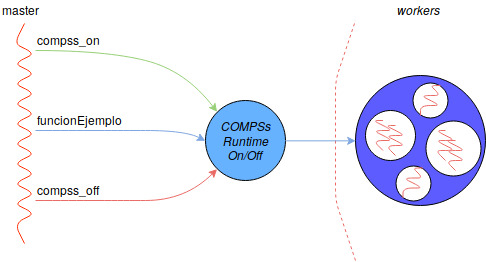
\includegraphics[scale=0.75]{sta-masterworker.jpg}
    \label{fig:masterworker_pool}
\end{figure}

La imagen muestra lo que sucede al ejecutar la aplicación de ejemplo de la sección \ref{compss_pm}, las líneas rojas curvas indican procesos (o bien \textit{threads}), lo importante sucede entre las flechas etiquetadas como compss\_on y compss\_off, la ejecución de la tarea. Se pide ejecutar la tarea funcionEjemplo al \textit{runtime} de \textit{COMPSs} y se decide en qué \textit{worker} se ejecutará. Hasta aquí podríamos pensar que es indéntico al \textit{thread-pool}. Nótese, que esto no es así, por el hecho de que no tenemos por qué hablar de una misma máquina, sino que pueden ser máquinas distintas, como se puede ver en el grupo de ordenadores de la imagen. 
\par\bigskip

En \textit{C/C++} existen dos tipos de \textit{worker}, uno \textbf{no persistente} y otro \textbf{persistente}. 

\begin{itemize}
 \item \textbf{No persistente:} Para cada tarea que se quiere ejecutar en uno de estos workers se debe crear el \textit{thread} y unas \textit{pipes} para hacer \textit{Inter-process communication} (IPC). %No sé si indagar en qué se pasa por las pipes, hmmm... qué se pasa por las pipes?
 \item \textbf{Persistente:} Este tipo de \textit{worker} se levanta una vez al inicio de la aplicación y espera recibir las tareas a ejecutar.
\end{itemize}


\subsection{OmpSs}

\textit{OmpSs} es desarrollado por el grupo \textit{PM - Programming Models}, perteneciente también al departamento de \textit{CS - Computer Science}.
\par\bigskip

\textit{OmpSs} es un modelo de programación que intenta explotar el paralelismo de las aplicaciones de una manera sencilla y aprovechando al máximo los recursos de la máquina\cite{duran2011ompss}. 
\par\bigskip
El nombre del modelo proviene de \textit{OpenMP} y \textit{StarSs} (modelo que desarrolló el \textit{BSC}), este integra funcionalidades presentes en ambos. Por parte de \textit{OpenMP} se quiere tomar la facilidad de paralelizar una aplicación secuencial insertando pragmas, y de \textit{StarSs} el modelo de ejecución basado en un \textit{thread-pool} y que permite la ejecución de código en más recursos que únicamente el procesador, es decir, que ofrece fácil gestión del resto de recursos de cómputo (\textit{GPUs}, \textit{FPGAs}, ...)\cite{sainz2014leveraging}\cite{filgueras2013heterogeneous}.

\subsubsection{Modelo de programación y ejecución}

El modelo de programación de \textit{OmpSs} se basa en la generación de tareas sencillamente insertando pragmas en código secuencial y a su vez facilitando la gestión de recursos heterogéneos. Veamos un pequeño ejemplo que muestre estas facultades.

\begin{lstlisting}[caption={Multiplicación de un bloque de una matriz utilizando GPUs.}, captionpos=b, label={lst:ompssmatmul.cc}, style=JStyle]
for (int i = 0; i < N; ++i) {
    for (int j = 0; j < N; ++j) {
        for (int k = 0; k < N; ++k) {
            #pragma omp target device(cuda) \
                               copy_deps    \
                               ndrange(2,N,N,32,32)
            #pragma omp task inout([N*N]C) in([N*N]A, [N*N]B)
            multiply_partitions_GPU(A[i*N+k], 
                                    B[k*N+j], 
                                    C[i*N+j], 
                                    n);
        }
    }
}
\end{lstlisting}

El código muestra una multiplicación de matrices por bloques. Con el primer pragma se indica que el dispositivo objetivo es una tarjeta gráfica que soporte \textit{CUDA}, y el segundo la declaración de una tarea y el tamaño de los bloques junto a las dependencias de esta.
\par\bigskip

El modelo de ejecución consiste en un \textit{thread-pool}, es decir, al generar tareas se escogerán \textit{threads} del \textit{pool} (entendámoslo como un conjunto de \textit{threads}) para ejecutarlas.
\par\bigskip

Cabe decir que para compilar una aplicación de \textit{OmpSs}, se utiliza el compilador \textit{source-to-source Mercurium} y el runtime \textit{Nanos++} para gestionar el paralelismo, es decir, la creación de tareas, sincronización entre estas, etc.

\subsection{COMPSs+OmpSs} 
\label{sec:compssompss}

Actualmente existe la posibilidad de desarrollar aplicaciones que utilicen \textit{OmpSs} dentro de \textit{COMPSs}. 
\par\bigskip
Para poder interactuar con el \textit{runtime} de \textit{OmpSs} \textit{Nanos++}, necesitamos gestionarlo nosotros manualmente o bien utilizar los pragmas que nos propone el modelo de programación y compilar con \textit{Mercurium}. Entonces, asegurándonos de registrar los \textit{workers} en el \textit{runtime} y compilando su código fuente con \textit{Mercurium} aseguramos la interacción con el \textit{runtime} y por lo tanto la integración de ambos modelos.

Es posible desarrollar aplicaciones, como ya se ha comentado, pero con ciertas restricciones. Las problemáticas aparecen con los dos tipos de \textit{worker} que hemos visto antes. Para el worker no persistente, no suele valer la pena debido a la granularidad de las tareas de \textit{OmpSs}. El \textit{overhead} proviene de crear el \textit{thread} del \textit{worker}, registrarlo en el \textit{runtime Nanos++} y levantar las \textit{pipes}. El persistente carece del \textit{overhead} de levantar las \textit{pipes} y el resto, vale la pena ya que el \textit{worker} persiste durante la ejecución de la aplicación. Pese a que el persistente mejora respecto al no persitente, hay problemas de migración de \textit{threads} entre aplicaciones cuando se ejecutan varias a la vez.
\par\bigskip

Estos problemas pretenden arreglarse integrando \textit{OmpSs-2}, que ofrece un \textit{runtime} nuevo llamado \textit{Nanos6} y nuevas características que vienen con este cambio como por ejemplo:

\begin{itemize}
\item \textbf{Liberación de las dependencias:} Las dependencias en esta versión se liberen de manera temprana, es decir, una vez una tarea acaba con un dato lo notifica al \textit{runtime} y este se encarga de notificar a las tareas que quedan libres de esta dependencia.
 \item \textbf{Relajación de las dependencias:} Ahora se pueden utilizar nuevos pragmas para determinar dependencias más suaves, no tan estrictas como en la versión anterior.
 \item \textbf{Ejecución de funciones de manera asíncrona:} La \textit{API} del nuevo \textit{runtime} \textit{Nanos6} permite ejecutar de manera asíncrona funciones en forma de tarea a partir de un puntero a una función.
\end{itemize}

Hemos listado las que de alguna manera eran clave para el proyecto, \textit{OmpSs-2} implementa muchas otras mejorías a parte de estas\cite{OmpSs2reference}. Una vez integrado, el proyecto estudiará si realmente han sido solucionadas las problemáticas anteriormente planteadas.

\section{Alcance del proyecto}

En esta sección se declaran las intenciones del proyecto (qué se pretende hacer), mediante una serie de requerimientos que harán que el proyecto pueda ser acabado con éxito, y unos objetivos que marcarán el desarrollo de este. También los posibles riesgos que surjan (y las soluciones de estos) y la metodología de trabajo que se llevará a cabo.

\subsection{Requerimientos}

 Los requerimientos necesarios para este proyecto son:

\begin{itemize}
 \item La nueva integración con \textit{OmpSs-2} no debe romper la actual compatibilidad con \textit{OmpSs}.
 \item El rendimiento de las aplicaciones desarrolladas con \textit{COMPSs+OmpSs-2} debe mejorar.
 \item Todas las modificaciones sobre \textit{COMPSs} deben ajustarse al grupo de \textit{Workflows and Distributed Computing}.
 \item Cualquier requerimiento impuesto (o aconsejado) por el \textit{BSC} formará parte de esta lista.
  
\end{itemize}

\subsection{Objetivos}

El objetivo principal de este proyecto es reformular la integración de \textit{COMPSs} con \textit{OmpSs} para solucionar los problemas actuales, ya sea integrándolo de nuevo pero esta vez con \textit{OmpSs-2} o bien idear otra manera de resolver las problemáticas. La siguiente lista muestra la posible descomposición de objetivos:

\begin{itemize}
  \item Aprender a utilizar la API (\textit{Application Programming Interface}) de \textit{Nanos6}.
  \item Eliminar o bien reducir las problemáticas planteadas en la sección   \ref{sec:compssompss}.
  \item Mejorar la gestión de recursos heterogéneos en las aplicaciones desarrolladas en \textit{COMPSs} integrando \textit{OmpSs-2}.
  \item En caso de conseguir el resto de objetivos plantear la integración en \textit{Java} y \textit{Python}.
\end{itemize}

\subsection{Riesgos}

Durante el desarrollo del proyecto pueden surgir problemas, para mejorar la reacción ante ellos listaremos los posibles riesgos y las respectivas soluciones.

\subsubsection{Problemas con el material de desarrollo}

Se podría romper el equipo en el cual se desarrolla el proyecto, pongamos que de una pantalla, un teclado y un ordenador se rompe el último. Se perdería todo el avance del proyecto, incluso documentación.
\par\medskip

\textbf{Solución:} Pese a que la pérdida del ordenador es importante, todo el código del proyecto será subido al \textit{GitLab} de \textit{WDS}, y la documentación al \textit{GitHub} personal del desarrollador, por lo cual se podría recuperar todo el  proyecto.

\subsubsection{Problemas con los clústers y supercomputadores}

Si por casualidad, caen los clústers y supercomputadores en los cuales se medirá el rendimiento del proyecto, se pararía la obtención de las métricas. 
\par\medskip

\textbf{Solución:} En este caso, como no resultaría lo mismo ejecutarlo en local en mi ordenador, debería optar por realizar otras tareas hasta que el equipo del \textit{BSC} solucione los inconvenientes.

\subsubsection{Aparición de errores en la implementación}

Cualquier proyecto esta lleno de errores en la implementación, hay que saber encontrarlos y solucionarlos lo más rápido posible, pero puede entorpecer el proyecto.
\par\medskip

\textbf{Solución:} Activaremos los \textit{flags} de \textit{debug} para poder evitar el mínimo error y en caso de su aparición utilizaremos \textit{gdb} (\textit{GNU Debugger}) para encontrarlo.

\subsubsection{Problemas con OmpSs/OmpSs-2}

Dado que se realizará una integración de otro proyecto del \textit{BSC} el desarrollador puede encontrarse con dificultades relacionadas con este a lo largo del proyecto.
\par\medskip

\textbf{Solución:} Después de haber intentado solucionarlo por sus propios medios se pondrá en contacto con el grupo de \textit{Programming Tools} con la descripción del error e intentos de solucionarlo.

\section{Metodología}

Para decidir la metodología a utilizar, hay que tener en cuenta que el proyecto consta únicamente de tres personas que se envolverán en él. El desarrollador, que hará todo el desarrollo tangible, el director y el codirector. 
\par\bigskip

La metodología que más se ciñe a las características del ``equipo'' es \textit{SCRUM}. Esta metodología forma parte de las populares (y bastante de moda) metodologías ágiles, consiste en planear al milímetro las tareas a realizar, y hacer una predicción de qué se conseguira hacer y que no en cortos periodos de tiempo llamados iteraciones. Además de estas predicciones, se consultará el estado del proyecto a diario, con cuestiones como ``¿Desde la última reunión que he conseguido?'', ``¿Desde entonces que haré para llegar a los objetivos de la iteración?'', ``¿Algún impedimento que no me permita alcanzar estos objetivos?''.
\par\bigskip

Esta metodología nos permitirá reaccionar rápidamente a los imprevistos, además de hacer un bueno monitoreo del estado del proyecto, por lo cual se ha decidido emplearla.

\subsection{Herramientas}

Para efectuar el seguimiento del proyecto junto a mi director y codirector, se empleará un \textit{workspace} de \textit{Slack} para las comunicaciones directas (decidir dónde y cuándo hacer las reuniones por ejemplo), y \textit{Trello} para gestionar las tareas a desempeñar en cada iteración. Como ya se ha mencionado anteriormente, para el control de versiones del proyecto, código y documentación se utilizará respectivamente \textit{GitLab} y \textit{GitHub}.

%\section{Planificación temporal}
\label{sec:planificacion}

Esta sección presenta como se utilizarán los aproximadamente cuatro meses de duración que tiene el proyecto, desde Febrero de 2019 hasta Junio de 2019. Se especificarán las tareas a realizar junto a su durada aproximada, teniendo en cuenta las posibles desviaciones en la realización de estas. Dado que cualquier desviación puede resultar en la alteración de la planificación, se debe tener en cuenta que la especificación que sigue no debe tomarse al pie de la letra, sino que debe reinterpretarse y modificarse siempre que sea necesario. 

\subsection{Especificación de las tareas}

Detallamos a continuación las tareas a realizar.

\subsubsection{GEP - Gestión de proyectos}

La asignatura GEP conforma el primer bloque del proyecto, se debe elaborar cuatro entregables que sinteticen la temática del proyecto, objetivos, como se realizará (metodología), definir las actividades, realizar un estudio de sostenibilidad y finalmente presentar este documento con soporte visual de manera oral ante un tribunal.

\begin{itemize}
 \item \textbf{Elaboración del primer entregable:} En este primer apartado se dará un contexto, el estado del arte del proyecto, los objetivos, requerimentos, riesgos y una metodología para desarrollar el proyecto en sí. La duración aproximada es de unas 24 horas.
 \item \textbf{Elaboración del segundo entregable:} En este apartado se definen las actividades y duración de estas. La duración aproximada es de 6 horas.
 \item \textbf{Elaboración del tercer entregable:} En este apartado se realizará la autoevaluación sobre la sostenibilidad además de un análisis sobre la gestión económica y la sostenibilidad del proyecto. La duración aproximada es de 18 horas.
 \item \textbf{Elaboración del cuarto entregable:} En este último apartado se preparará una presentación oral y se confeccionará el documento final, que serán los tres anteriores revisados y corregidos con la orientación del \textit{feedback} del profesor de GEP, director y codirector. La duración aproximada es de 12 horas.
\end{itemize}

Con estos cuatro apartados se finaliza el GEP. En princpio, la duración estipulada del GEP es de 75 horas, la suma de las horas que hemos creído que durarían es de 60 horas, esta diferencia nos proporcionará cierto margen para corregir y mejorar los entregables. Para realizar esta actividad, se empleará un ordenador, \textit{GitHub} para subir la documentación, \textit{Kile} para redactar el documento en \textit{LaTeX},\textit{Trello} para organizar las actividades en forma de tarjetas, \textit{Gantter} para elaborar el diagrama de \textit{Gantt} y \textit{Google Drive}.

\subsubsection{Uso de la API de Nanos6}

Para poder llevar acabo exitosamente la integración, se necesita entender qué hace y saber utilizar la \textit{API} de \textit{Nanos6}. Requiere mirar documentación e interactuar con los desarrolladores de \textit{Nanos6}. 
\par\bigskip

Queremos aprender a utilizar la llamada \textit{nanos6\_spawn\_function}, que nos permitirá ejecutar una función como tarea. Para poder utilizarla, necesitamos levantar el \textit{runtime} de manera manual en un programa compilado con \textit{gcc} (\textit{GNU C Compiler}) o bien \textit{g++} cuando se utilice \textit{C++}, y efectuar la llamada a una función externa compilada con \textit{mcc} (\textit{Mercurium}), ya que estará anotada con pragmas de \textit{OmpSs-2}.
\par\bigskip

El tiempo aproximado para realizar esta tarea es de 60 horas. Los recursos necesarios son un ordenador con un compilador nativo de \textit{C}, otro de \textit{C++}, y \textit{Mercurium} y \textit{Nanos6} instalados. 

\subsubsection{Integrar OmpSs-2 en el binding de C/C++}

La tarea principal que da sentido al proyecto es esta, comprende el estudio y la integración de \textit{OmpSs-2} en el \textit{binding} de \textit{C/C++}. Requiere del estudio de la estructura interna de \textit{COMPSs} por una banda y del \textit{binding} por otra, con tal de saber dónde se podría inicializar el \textit{runtime} de \textit{Nanos6} y cuándo se debería apagar. También se necesita hacer la llamada a la \textit{API} en el \textit{worker}, cosa que habrá que estudiar también dónde situar.
\par\bigskip

El primer paso consistirá en analizar dónde tendría más sentido que hagamos la gestión del \textit{runtime} de \textit{Nanos6}, y cómo hacerla. Para esto tendremos que dar un repaso al código de \textit{COMPSs} y determinar qué hace cada componente de este. 
%\par\bigksip

En segundo lugar se deberá implementar toda la gestión. Se deberá también estudiar dónde se debería hacer la llamada a la \textit{API}, y por verificar el funcionamiento de la integración, que será de seguro lo más complejo y lo que más tiempo requerirá.
%\par\bigskip

Esta tarea es la que más tiempo nos llevará, ya que será el primer intento serio de integrarlo todo, pero nos aportará conocimiento pleno de como funciona y por lo tanto facilidad para trabajar en futuras ampliaciones. La duración será aproximadamente de 96 horas. Los recursos necesarios son un ordenador con \textit{COMPSs} instalado, un compilador nativo de \textit{C}, otro de \textit{C++}, y \textit{Mercurium} y \textit{Nanos6} instalados.

\subsubsection{Estudiar la integración de OmpSs-2 en Java y binding de Python}

En caso de que la primera integración haya funcionado, se estudiará la posibilidad de hacer lo mismo con \textit{Java} y el \textit{binding} de \textit{Python}. Consistirá exactamente de los mismos pasos, y puede ayudar a mejorar la implementación anterior. La duración estimada de esta tarea dependerá de si se decide realizar o no esta actividad. Mínimo se emplearán 15 horas en el estudio preliminar, y en caso de realizar la integración, 78 horas más, es decir, 15 horas o bien 93 horas. Pese a que la tarea es muy similar a la anterior, el tiempo previsto es algo menor por el hecho de que ya se ha podido realizar una integración y la implementación debería ser parecida. Los recursos necesarios son un ordenador con \textit{COMPSs} instalado, un compilador nativo de \textit{C}, otro de \textit{C++}, y \textit{Mercurium} y \textit{Nanos6} instalados.

\subsubsection{Estudio previo del rendimiento}

Dado que este proyecto parte de la premisa de resolver unos problemas concretos con el rendimiento, se efectúa un estudio muy concreto hacia estos problemas para ver si están resueltos o no. Que este estudio vaya mal o no, no afecta realmente al proyecto, ya que se intentará ver si \textit{OmpSs-2} mejora respecto a \textit{OmpSs} de todas formas.

\subsubsection{Desarrollo de una aplicación que use COMPSs+OmpSs-2}

En esta tarea se quiere desarrollar una aplicación que haga uso de \textit{COMPSs+OmpSs-2} con tal de estudiar después el rendimiento de la integración. La aplicación no puede ser cualquiera, ya que no toda aplicación mejorará su rendimiento conforme añadamos recursos heterogéneos. Dado que aún hay mucho margen, se ideará más adelante cuál será la aplicación a desarrollar. El tiempo que se empleará en esta tarea es de aproximadamente 84 horas. Los recursos necesarios son un ordenador con \textit{COMPSs} instalado, un compilador nativo de \textit{C}, otro de \textit{C++}, y \textit{Mercurium} y \textit{Nanos6} instalados.

\subsubsection{Estudio del rendimiento}

Utilizando la aplicación desarrollada en la tarea anterior estudiaremos el rendimiento de la integración, haremos uso de herramientas del \textit{BSC} como por ejemplo \textit{Extrae} y \textit{Paraver}, desarrolladas por el grupo \textit{Performance Tools} que nos permitirán extraer trazas para las tareas que ejecuten los \textit{workers} una vez la aplicación haya acabado y después visualizarlas. También haremos uso de opciones de \textit{COMPSs} para medir cuánto tarda cada tarea enviada a un nodo.
\par\bigskip

Estudiar el rendimiento incluirá intentar optimizar al máximo todas las pérdidas de rendimiento en la medida de lo posible, por lo cual el tiempo aproximado para llevarla a cabo, es de 84 horas. Los recursos necesarios son un ordenador con las herramientas mencionadas anteriormente instaladas, \textit{COMPSs} instalado, un compilador nativo de \textit{C}, otro de \textit{C++}, y \textit{Mercurium} y \textit{Nanos6} instalados.

\subsubsection{Redactar la memoria}

Por último se deberá redactar la memoria del proyecto además de preparar todo el material audiovisual para la defensa de este. La duración de esta actividad será de unas 72 horas. Los recursos que se utilizarán son \textit{Kile} para redactar el documento en \textit{LaTeX}, \textit{GitHub} para guardar la documentación y \textit{LibreOffice} para el apoyo audiovisual que se utilizará durante la defensa.

\subsection{Dependencias}

La siguiente tabla define la relación de dependencia entre las tareas que conciernen a la gestión del proyecto.

\begin{table}[H]
\centering
 \begin{tabular}{|| l | l ||}
    \hline  
    Tarea dependiente & Tarea predecesora \\
    \hline\hline
    Contexto & - \\
    \hline
    Estado del arte & Contexto \\
    \hline
    Objetivos, requerimentos, riesgos & Estado del arte \\
    \hline
    Metodología & Objetivos, requerimentos, riesgos \\
    \hline
    Definir actividades & Metodología \\
    \hline
    Estimar tiempos & Definir actividades \\
    \hline
    Autoevaluación sobre la sostenibilidad & Estimar tiempos \\
    \hline
    Análisis del proyecto & Autoevaluación sobre la sostenibilidad \\
    \hline
    Confeccionar documento final & Análisis del proyecto \\
    \hline
    Preparar presentación & Confeccionar documento final \\
    \hline
 \end{tabular}
 \caption{Relación de dependencia para las tareas de la gestión del proyecto.}
 \label{table:1}
\end{table}

La tabla anterior muestra la relación de dependencia, se respetará esta relación ya que las tareas a elaborar se agrupan y tienen fecha de entrega por separado. 

\begin{table}[H]
 \centering
 \begin{tabular}{|| l | l ||}
    \hline  
    Tarea dependiente & Tarea predecesora \\
    \hline\hline
    Uso de la API Nanos6 & GEP \\
    \hline
    Integrar OmpSs-2 en C/C++ & Uso de la API \\
    \hline
    Integrar OmpSs-2 en Java & Integrar OmpSs-2 en C/C++ \\
    \hline
    Integrar OmpSs-2 en Python & Integrar OmpSs-2 en Java \\
    \hline
    Estudio previo del rendimiento & Integrar OmpSs-2 en Python \\
    \hline
    Desarrollo aplicación COMPSs+OmpSs-2 & Estudio previo del rendimiento \\
    \hline
    Estudio del rendimiento & Desarrollo aplicación COMPSs+OmpSs-2 \\
    \hline
    Redactar la memoria & Estudio del rendimiento \\
    \hline
 \end{tabular}
    \caption{Relación de dependencia para las tareas de implementación del proyecto.}
    \label{table:2}
\end{table}

Salvo por algún motivo que implique bloquear una tarea, no se deberán adelantar tareas dependientes a las predecesoras, entre estos posibles motivos se contemplan errores en la implementación que nos bloqueen y se puedan ir haciendo otras cosas y cambios generales en las tareas a realizar.

\subsection{Estimación temporal de las tareas y recursos necesarios}

En el momento en el que se han enumerado y explicado las tareas se ha comentado la duración temporal y los recursos necesarios para cada actividad. En las siguientes dos secciones se recopilan estos datos en forma de tabla.

\subsection{Estimación temporal de las tareas}

\begin{table}[H]
 \centering
 \begin{tabular}{|| l | l ||}
  \hline
  Tarea & Estimación temporal (horas) \\
  \hline\hline
   Gestión del proyecto & 60 \\%& GitHub, Kile, Trello, Gantter, Google Drive \\
   \hline
   Uso de la API Nanos6 & 60 \\%& Compilador de C y C++, Mercurium, Nanos6 \\
   \hline
   Integrar OmpSs-2 en C/C++ & 96 \\%& COMPSs, Compilador de C y C++, Mercurium, Nanos6 \\
   \hline
   Integrar OmpSs-2 en Java y Python & 93 \\%& COMPSs, Compilador de C y C++, Mercuirum, Nanos6 \\
   \hline
   Desarrollo aplicación COMPSs+OmpSs-2 & 84 \\%& COMPSs, Compilador de C y C++, Mercurium, Nanos6 \\
   \hline
   Estudio del rendimiento & 84 \\%& COMPSs, Compilador de C y C++, Mercurium, Nanos6 \\
   \hline
   Redactar la memoria & 72 \\%& GitHub, Kile, LibreOffice \\
  \hline
  Total & 549 \\
  \hline
 \end{tabular}
 \caption{Estimación temporal de las tareas.}
\end{table}

En los apéndices 

\subsection{Recursos necesarios para las tareas}

\begin{table}[H]
 \centering
 \begin{tabular}{| l | l |}
 \hline
 Tarea & Recursos necesarios \\
 \hline\hline  
 Gestión del proyecto & GitHub, Kile, Trello, Gantter, Google Drive \\
 \hline
 Uso de la API Nanos6 & Compilador de C y C++, Mercurium, Nanos6 \\
 \hline
 Integrar OmpSs-2 en C/C++ & COMPSs, Compilador de C y C++, Mercurium, Nanos6 \\
 \hline
 Integrar OmpSs-2 en Java y Python & COMPSs, Compilador de C y C++, Mercurium, Nanos6 \\
 \hline
 Estudio del rendimiento & COMPSs, Compilador de C y C++, Mercurium, Nanos6 \\
 \hline
 Redactar la memoria & GitHub, Kile, LibreOffice \\
 \hline
 \end{tabular}
 \caption{Recursos necesarios para las tareas.}
\end{table}

En la tabla anterior, se muestran los recursos estrictamente necesarios para realizar la tarea, sin embargo, se ofrece ahora una lista de los recursos \textit{hardware} y \textit{software} que se utilizarán para la realización del proyecto en general. Además hay que tener en cuenta todos los recursos humanos necesarios.

\subsubsection{Recursos hardware}

\begin{itemize}

 \item \textbf{Ordenador portátil:} Proporcionado por el \textit{BSC}, Dell Latitude 7480 Intel® Core™ i7-6650U Processor (Dual Core, 4M Cache, 2.2GHz,15W, vPro), 512GB SSD (\textit{Solid State Drive}), Intel® HD Graphics 540 y 16 GB de memoria \textit{RAM}.
 
 \item \textbf{Pantalla:} Es habitual la configuración de portátil con una pantalla para simular una torre, la pantalla externa es también Dell, el modelo Professional P2217H.
 
 \item \textbf{Periféricos:} Todos los periféricos, ratón y teclado en este caso.
 
 \item \textbf{Clústers:} Con tal de medir el rendimiento ejecutando la aplicación que se desarrollará haciendo uso de la integración, necesitaremos un clúster con una arquitectura heterogénea. En la lista de candidatos se encuentran \textit{MinoTauro} y \textit{CTE-Power}, ambos están dotados de nodos que contienen \textit{CPUs} y \textit{GPUs}, se aprofundizará más en sus caracterísitcas en el momento de medir el rendimiento.
 
 \item \textbf{Puesto de trabajo:} El equipo de \textit{WDC} se encuentra en el edificio \textit{K2M}, allí es donde el desarrollador tendrá un puesto de trabajo y podrá desarrollar la mayoría del proyecto.
 
\end{itemize}

\subsubsection{Recursos software}

\begin{itemize}
    \item \textbf{Ubuntu 18.04:} Con tal de desarrollar se necesita un sistema operativo, el portátil tendrá instalado \textit{Ubuntu 18.04}.

    \item \textbf{GitHub y GitLab:} Para efectuar un control de versiones sencillo y eficaz, se utilizará el \textit{GitHub} personal del desarrollador para gestionar la documentación y el \textit{GitLab} del grupo \textit{WDC} para gestionar el código.

    \item \textbf{Editores: } Para editar código en \textit{Java} se utilizará \textit{IntelliJ IDEA}, para \textit{Python} \textit{PyCharm}, ambos de \textit{JetBrains}, y para C y C++ se utilizará \textit{Vim}.

    \item \textbf{Terminal: } La gran parte del tiempo se pasará entre terminales haciendo implementaciones y probando su funcionamiento, para hacer uso de un terminal se utilizará el emulador de terminales \textit{Terminator}.

    \item \textbf{Planificación y organización: } Para hacer el diagrama de \textit{Gantt} se ha utilizado \textit{Gantter} como extensión para \textit{Google Drive}. Además para organizarse y emplear la metodología \textit{SCRUM} se utilizará \textit{Trello}.

    \item \textbf{Compiladores y gestores de proyectos: } Para compilar código en C y C++ se utilizará \textit{gcc} y \textit{g++} respectivamente, para todo código que use \textit{OmpSs-2} se utilizará \textit{Mercurium}. El proyecto de \textit{COMPSs} está gestionado con \textit{Maven}, de esta manera se pueden generar todos los ficheros de \textit{Java} de manera sencilla. 
    
    \item \textbf{Software del proyecto: } Para poder desarrollar el proyecto, se precisará de una instalación de \textit{COMPSs}, \textit{Nanos6} y \textit{Mercurium}. Además, para medir el rendimiento se precisará de \textit{Extrae} y \textit{Paraver}. Con fines de \textit{debugging} se utilizará \textit{gdb}.

    \item \textbf{Editores de texto: } Para escribir el \textit{LaTeX} se utilizará \textit{Kile}.
\end{itemize}

\subsubsection{Recursos humanos}

\begin{itemize}
 \item \textbf{Director y codirector: } Efectuarán el seguimiento del proyecto de manera rutinaria y ayudarán a que el desarrollador sea capaz de llevarlo a cabo. 
 \item \textbf{Soporte: } Al utilizar \textit{software} de diversos proyectos, todas las personas que ayuden al desarrollador a solucionar problemas son recursos necesarios del proyecto.
 \item \textbf{Desarrollador: } Persona encargada de llevar a cabo en ultima instancia el proyecto.
\end{itemize}

\subsection{Valoración de alternativas y plan de acción}

En un proyecto de este tipo, es probable que haya desviaciones respecto el plan original. Esto es normal, tan sólo hay que saber cómo actuar ante estas desviaciones. Cualquier error en una implementación puede acarrear tiempo de más para solucionarlo, e incluso algo que se implementó hace mucho puede influir en las del futuro, por ello nuestra planificación intenta ser flexible, aún así, debemos planear como actuar en estos casos.

\begin{itemize}
 \item Si una tarea dura menos de lo esperado, sencillamente hay que coger la siguiente de la planificación y empezar a hacerla. Que una tarea dure menos que otra nos puede aportar un margen de acción muy útil.
 \item Si una tarea dura más tiempo de lo esperado, habrá que planteárselo de dos maneras, o bien se acorta otra tarea con tal de ajustarnos a la planificación o bien se intentan reducir lo mínimo posible los objetivos del proyecto para poderlo acabar en el tiempo establecido.
\end{itemize}

La tarea que más tiempo puede llevar dada la aparición de imprevistos es la de integrar \textit{OmpSs-2} en el \textit{binding} de C. Dado que la documentación aún está en una fase un tanto primeriza y no siempre tenemos por qué contar con el apoyo de soporte, por lo cuál habrá que invertir tiempo extra en ese caso. 
\par\medskip
El resto de tareas van un poco de la mano de esta anterior, no debería haber ninguna complicación extra. Como mucho en el estudio del rendimiento podemos encontrar resultados que no nos gusten o no acaben de agradar del todo, pero es parte del proyecto, se intentará mejorar dentro del tiempo estipulado. 
\par\medskip
Por tanto, siempre que falte tiempo para realizar una tarea se intentará equilibrar entre el resto, ya que el riesgo de sufrir un imprevisto es bastante bajo.
\par\bigskip
Para ser más previsores, en las reuniones de seguimiento se intentarán prever estos posibles problemas durante la realización del proyecto. 



















\section{Gestión económica y sostenibilidad}

Cuando se desarrolla un proyecto siempre hay un cierto impacto ambiental, económico, social. Cómo el proyecto impacta sobre estas tres componentes indica cuánto de sostenbile es el proyecto. Aunque \textit{a priori} desconocemos las técnicas para medir el impacto, se conseguirá hacer una aproximación del impacto del proyecto. 

\subsection{Análisis de la sostenibilidad}

\subsection{Getsión económica}

\subsubsection{Presupuesto}



%\printbibliography
\end{document}
